\documentclass[10pt]{beamer}
\usefonttheme{professionalfonts}
%\usetheme{CambridgeUS}
%
% Choose how your presentation looks.
%
% For more themes, color themes and font themes, see:
% http://deic.uab.es/~iblanes/beamer_gallery/index_by_theme.html
%
\mode<presentation>
{
  \usetheme{default}      % or try Darmstadt, Madrid, Warsaw, ...
  \usecolortheme{beaver} % or try albatross, beaver, crane, ...
  \usefonttheme{default}  % or try serif, structurebold, ...
  \setbeamertemplate{navigation symbols}{}
  \setbeamertemplate{caption}[numbered]
} 

\usepackage[english]{babel}
\usepackage[utf8x]{inputenc}
\usepackage{tikz}
\usepackage{pgfplots}
\usepackage{array}  % for table column M
\usepackage{makecell} % to break line within a cell
\usepackage{verbatim}
\usepackage{graphicx}
\usepackage{epstopdf}
\usepackage{amsfonts}
\usepackage{xcolor}
%\captionsetup{compatibility=false}
%\usepackage{dsfont}
\usepackage[absolute,overlay]{textpos}
\usetikzlibrary{calc}
\usetikzlibrary{pgfplots.fillbetween, backgrounds}
\usetikzlibrary{positioning}
\usetikzlibrary{arrows}
\usetikzlibrary{pgfplots.groupplots}
\usetikzlibrary{arrows.meta}
\usetikzlibrary{plotmarks}

\usepgfplotslibrary{groupplots}
\pgfplotsset{compat=newest} 
%\pgfplotsset{plot coordinates/math parser=false}

\usepackage{hyperref}
\hypersetup{
    colorlinks=true,
    linkcolor=blue,
    filecolor=magenta,      
    urlcolor=cyan,
}

\definecolor{matlabcomment}{RGB}{34,139,34}

\pgfmathdeclarefunction{gauss}{1}{%
	\pgfmathparse{1/(sqrt(2*pi))*exp(-((#1)^2)/2)}%
}

\pgfmathdeclarefunction{laplacian}{2}{%
	\pgfmathparse{1/(#2*2)*exp(-(abs(x-#1))/(#2))}%
}

\pgfmathdeclarefunction{pretty_func}{1}{%
	\pgfmathparse{cos(deg(#1/2)) - sin(deg(#1)) + cos(deg(#1/2)-45) - sin(deg(#1/4)-154)}%
}

\pgfplotsset{
	dirac/.style={
		mark=triangle*,
		mark options={scale=2},
		ycomb,
		scatter,
		visualization depends on={y/abs(y)-1 \as \sign},
		scatter/@pre marker code/.code={\scope[rotate=90*\sign,yshift=-2pt]}
	}
}

\tikzset{
	invisible/.style={opacity=0},
	visible on/.style={alt={#1{}{invisible}}},
	alt/.code args={<#1>#2#3}{%
		\alt<#1>{\pgfkeysalso{#2}}{\pgfkeysalso{#3}} % \pgfkeysalso doesn't change the path
	},
}

\newcommand\PlotSampledSpectrum[4]{%
	\def\fs{#2}%
	\def\fmax{#3}%
	\def\ros{#4}%
	\input{#1}%
}

\pgfmathdeclarefunction{invgauss}{2}{%
	\pgfmathparse{sqrt(-2*ln(#1))*cos(deg(2*pi*#2))}%
}

\tikzset{
	declare function={
		sinc(\x) = (and(\x!=0, 1) * (sin(deg(pi*\x))/(pi*\x)) +
		(and(\x==0, 1) * 1);
	}
}

\DeclareMathOperator{\E}{\mathbb{E}} % expectation

\newcolumntype{M}[1]{>{\centering\arraybackslash}m{#1}}

\definecolor{blue2}{RGB}{51, 105, 232}  
\definecolor{red2}{RGB}{213, 15, 37}  
\definecolor{green2}{RGB}{0, 153, 37}  
\definecolor{green3}{rgb}{0.1922, 0.6392, 0.3294}% 
\definecolor{yellow2}{RGB}{238, 178, 17} 
\definecolor{gray2}{RGB}{102, 102, 102}
\definecolor{orange2}{RGB}{230, 85, 13}

% Qualitative pallete set1 from www.ColorBrewer.org
\definecolor{Qred}{RGB}{228,26,28}
\definecolor{Qblue}{RGB}{55,126,184}
\definecolor{Qgreen}{RGB}{77,175,74}
\definecolor{Qpurple}{RGB}{152,78,163}
\definecolor{Qorange}{RGB}{255,127,0}
\definecolor{Qyellow}{RGB}{255,255,51}
\definecolor{Qbrown}{RGB}{166,86,40}
\definecolor{Qpink}{RGB}{247,129,191}
\definecolor{Qgray}{RGB}{153,153,153}

\newcommand\PlotGaussianCF[4]{%
	\def\sig{#2}%
	\def\ws{#3}%
	\def\cap{#4}
	\input{#1}%
}

%% 
\title[EE 264]{Properties of LTI Systems}
\author{Jose Krause Perin}
\institute{Stanford University}
\date{July 18, 2017}

\begin{document}

\begin{frame}
  \titlepage
\end{frame}

%
%\begin{frame}{Announcements}
%	\begin{itemize}
%		\item Homework \#2 due today
%		\item Homework \#3 will be released today and it is due next Thursday
%	\end{itemize}
%\end{frame}

%
\begin{frame}{Last lecture}
\begin{itemize}
	\item Quantization is unavoidable in DSP systems
	\item Although quantization is a nonlinear operation on a signal, it is a linear operation on the signal PDF (area sampling)
	\item The probabilistic interpretation of quantization allows us to model the quantization error as an uniformly distributed random process (linear noise model)
	\item Using this linear noise model, we simply replace quantizers by noise sources of average power $\sigma_e^2 = \Delta^2/12$
	\item Quantization noise is assumed white (samples are uncorrelated)
	\item Every extra bit of resolution in a quantizer improves the SNR by 6.02 dB
	\item The signal amplitude must be matched to the dynamic range of the quantizer, otherwise there'll be excessive clipping or some bits won't be used
	\item Noise shaping is a strategy that minimizes quantization noise in A-to-D and D-to-A converters. The goal is to shape the quantization noise PSD, so that most of the noise power falls outside the signal band
	\item Noise shaping requires oversampling to minimize noise aliasing
\end{itemize}
\end{frame}

%
\begin{frame}{Practice and theory}
\begin{block}{In practice}
	\begin{center}
		\resizebox{\linewidth}{!}{\def\layersep{1.5cm}
\def\outsep{0.7cm}
\def\dy{1.25}

\begin{tikzpicture}[->, >=stealth, shorten >= 0pt, draw=black!50, node distance=\layersep, font=\sffamily]
    \tikzstyle{node}=[circle,fill=black,minimum size=2pt,inner sep=0pt]
    \tikzstyle{block}=[draw=black,rectangle,fill=none,minimum size=1.5cm, inner sep=0pt]
    \tikzstyle{annot} = []

	\node[node] (xc) at (0, -\dy cm) {};
    \node[block] (ADC) at (1*\layersep, -\dy cm) {ADC};
    \node[block, text width = 2.5cm, align= center] (DSP) at (3*\layersep, -\dy cm) {Digital Signal Processor};
    \node[block] (DAC) at (5*\layersep, -\dy cm) {DAC};
	\coordinate (yc) at (6*\layersep, -\dy cm) {};
	
	\coordinate (mid1) at ($(ADC.east)!0.5!(DSP.west)$) {};
	\coordinate (mid2) at ($(DSP.east)!0.5!(DAC.west)$) {};
		
    \path (xc) edge (ADC);
    \path (ADC) edge (DSP);
    \path (DSP) edge (DAC);
    \path (DAC) edge (yc);
    
    \node[above = 0.5mm of mid1] {$x[n]$};
    \node[above = 0.5mm of mid2] {$y[n]$};
    \node[above = 0mm of xc, text width = 1cm, align=center] {$x_c(t)$};
    \node[above = 0mm of yc, text width = 1cm, align=center] {$y_c(t)$}; 
    

\end{tikzpicture}}
	\end{center}
\end{block}

\begin{block}{DSP theory}
	\begin{center}
		\resizebox{\linewidth}{!}{\def\layersep{2cm}
\def\outsep{0.7cm}
\def\dy{1.25}

\begin{tikzpicture}[->, >=stealth, shorten >= 0pt, draw=black!50, node distance=\layersep, font=\sffamily]
    \tikzstyle{node}=[circle,fill=black,minimum size=2pt,inner sep=0pt]
    \tikzstyle{block}=[draw=black,rectangle,fill=none,minimum size=1.5cm, inner sep=0pt]
    \tikzstyle{annot} = []

	\node[node] (xc) at (0, -\dy cm) {};
    \node[block] (ADC) at (1*\layersep, -\dy cm) {C-to-D};
    \node[block, text width = 2cm, align= center] (DSP) at (3*\layersep, -\dy cm) {LTI \\ System};
    \node[block] (DAC) at (5*\layersep, -\dy cm) {D-to-C};
	\coordinate (yc) at (6*\layersep, -\dy cm) {};
	
	\coordinate (mid1) at ($(ADC.east)!0.5!(DSP.west)$) {};
	\coordinate (mid2) at ($(DSP.east)!0.5!(DAC.west)$) {};
		
    \path (xc) edge (ADC);
    \path (ADC) edge (DSP);
    \path (DSP) edge (DAC);
    \path (DAC) edge (yc);
    
    \node[above = 0.5mm of mid1] {$x[n]$};
    \node[below = 0.5mm of mid1] {$X(e^{j\omega})$};
    \node[above = 0.5mm of mid2] {$y[n]$};
    \node[below = 0.5mm of mid2] {$Y(e^{j\omega})$};
    \node[above = 0mm of xc, text width = 1cm, align=center] {$x_c(t)$};
    \node[below = 0mm of xc, text width = 1cm, align=center] {$X_c(j\Omega)$};
    \node[above = 0mm of yc, text width = 1cm, align=center] {$y_r(t)$}; 
    \node[below = 0mm of yc, text width = 1cm, align=center] {$Y_r(j\Omega)$};
    \node at ($(DSP.south)-(0, 0.25cm)$) {$h[n] \leftrightarrow H(e^{j\omega})$};
\end{tikzpicture}}
	\end{center}
\end{block}
\end{frame}

%
\section{Outline}
\begin{frame}{Outline}
\begin{itemize}
	\item Magnitude and phase response
	\item Phase and group delay
	\item Pole-zero plot and the frequency response
	\item All-pass systems
	\item Linear phase systems
	\item Generalized linear phase systems
	\item Minimum phase systems
\end{itemize}
\end{frame}

\begin{frame}{Magnitude and phase response}
Recall that complex exponentials are \textbf{eigenfunctions} of LTI systems
\begin{equation*}
\mathrm{LTI}\{e^{j\omega n}\} = H(e^{j\omega})e^{j\omega n}
\end{equation*}

$H(e^{j\omega})$ is the corresponding \textbf{eigenvalue} of $e^{j\omega n}$

$H(e^{j\omega})$ tell us by how much the LTI system \textbf{scaled} and \textbf{delayed} $e^{j\omega n}$

\begin{equation*}
H(e^{j\omega}) = \underbrace{|H(e^{j\omega})|}_{\text{Magnitude}}\exp(j\underbrace{\angle H(e^{j\omega})}_{\text{Phase}})
\end{equation*}

\pause
\texttt{>> freqz(a, b)}
\vspace{-0.25cm}
\begin{center}
	\begin{tikzpicture}
	\node (img1) {\resizebox{0.5\linewidth}{!}{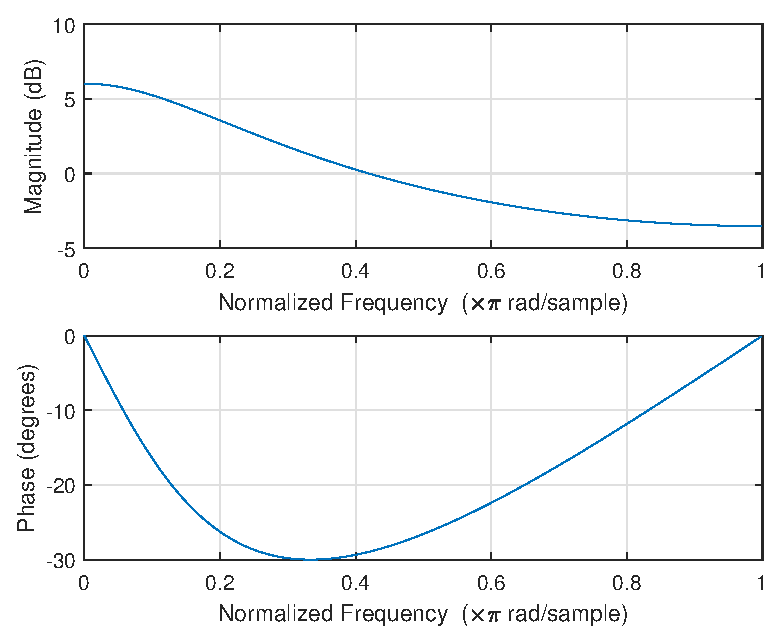
\includegraphics{figs/first_order_sys_freqz.eps}}};
	\node at ($(img1.north east) -(2cm, 0.75cm)$) {$20\log_{10}(|H(e^{j\omega})|)$};
	\node at ($(img1.east)-(2.9cm, 0.5cm)$) {$\angle H(e^{j\omega}) = \arg(H(e^{j\omega}))$};
	\end{tikzpicture}
\end{center}
\end{frame}

\begin{frame}{Phase unwrapping}
Depending on how the phase is calculated, we may need to perform an operation called phase unwrapping

Phase wrapping causes jumps of $\pm\pi$ in the phase response.

Most scientific programming languages should have a function named \texttt{arg} or \texttt{atan2}, which can be used to calculate the argument of a complex number.

\end{frame}

\begin{frame}{Group delay}
	Group delay is defined as 
	\begin{equation*}
	\tau_g(\omega) \equiv -\dfrac{d}{d\omega}\mathrm{arg} H(e^{j\omega}) \tag{group delay}
	\end{equation*}
	
	It measures by how much frequency $\omega$ is delayed. Delay in continuous-time means time and in discrete time it means samples.
	
	\textbf{Example:} If a system has linear phase:
	\begin{equation*}
		\mathrm{arg} H(e^{j\omega}) = -\omega n_d \tag{\textbf{linear phase}}
	\end{equation*} 
	
	Then, the group delay is constant:
	\begin{equation*}
	\tau_g(\omega) = -\dfrac{d}{d\omega}(-\omega n_d) = n_d \tag{\textbf{constant group delay}}
	\end{equation*} 
	
	\textbf{Conclusion:} Linear-phase systems delay all frequencies equally.	
\end{frame}


\begin{frame}{An interesting example}
	Consider the \underline{causal} LTI system defined by the following $z$-transform
	\begin{align*}
	&H(z) = \\ &\bigg(\frac{(1-0.98e^{j0.8\pi}z^{-1})(1-0.98e^{-j0.8\pi}z^{-1})}{(1-0.8e^{j0.4\pi}z^{-1})(1-0.8e^{-j0.4\pi}z^{-1})}\bigg)\prod_{k=1}^4\bigg(\frac{(c_k^* -z^{-1})(c_k -z^{-1})}{(1 -c_kz^{-1})(1 -c_k^*z^{-1})}\bigg)^2
	\end{align*}
	where $c_k = 0.95e^{j(0.15\pi + 0.02\pi k)}$
	
	It has the following pole-zero diagram:
	
	\begin{center}
		\resizebox{0.5\linewidth}{!}{\begin{tikzpicture}
\begin{axis}[
axis equal,
axis lines*=middle,
enlargelimits = false, clip=true,
xmin=-1.39,
xmax=1.39,
ymin=-1.10,
ymax=1.10,
axis line style={->,>=stealth},
xlabel={$\mathrm{Re}\{z\}$},
ylabel={$\mathrm{Im}\{z\}$},
every axis x label/.style={
at={(ticklabel* cs:1)},
anchor=north,
},
every axis y label/.style={
at={(ticklabel* cs:1)},
anchor=south,
},
xmajorgrids,
ymajorgrids,
every outer y axis line/.append style={white!15!black},
every y tick label/.append style={font=\color{white!15!black}},
legend style={draw=white!15!black,fill=white,legend cell align=left}]
\draw (axis cs:0,0) circle [black!50, dashed, line width=2pt, radius=1];
\addplot [line width=1pt,mark=x, only marks, mark size = 3pt]
table[row sep=crcr]{
	0.24721 0.76085 \\
	0.24721 -0.76085 \\
	0.8177 0.48359 \\
	0.78573 0.53398 \\
	0.75065 0.58226 \\
	0.71261 0.62825 \\
	0.8177 0.48359 \\
	0.78573 0.53398 \\
	0.75065 0.58226 \\
	0.71261 0.62825 \\
	0.8177 -0.48359 \\
	0.78573 -0.53398 \\
	0.75065 -0.58226 \\
	0.71261 -0.62825 \\
	0.8177 -0.48359 \\
	0.78573 -0.53398 \\
	0.75065 -0.58226 \\
	0.71261 -0.62825 \\
};

\addplot [line width=1pt,mark=*, only marks, mark size = 3pt, mark options={fill=white}]
table[row sep=crcr]{
	-0.79284 0.57603 \\
	-0.79284 -0.57603 \\
	0.90604 -0.53583 \\
	0.87061 -0.59167 \\
	0.83174 -0.64517 \\
	0.78959 -0.69612 \\
	0.90604 -0.53583 \\
	0.87061 -0.59167 \\
	0.83174 -0.64517 \\
	0.78959 -0.69612 \\
	0.90604 0.53583 \\
	0.87061 0.59167 \\
	0.83174 0.64517 \\
	0.78959 0.69612 \\
	0.90604 0.53583 \\
	0.87061 0.59167 \\
	0.83174 0.64517 \\
	0.78959 0.69612 \\
};

% Annotations
\node[align=left, anchor=south] at(axis cs: 0.65, -0.67) {\scriptsize $2$};
\node[align=left, anchor=south] at(axis cs: 0.68, -0.61) {\scriptsize $2$};
\node[align=left, anchor=south] at(axis cs: 0.74, -0.56) {\scriptsize $2$};
\node[align=left, anchor=south] at(axis cs: 0.78, -0.5) {\scriptsize $2$};

\node[align=left, anchor=south] at(axis cs: 0.64, 0.5) {\scriptsize $2$};
\node[align=left, anchor=south] at(axis cs: 0.68, 0.45) {\scriptsize $2$};
\node[align=left, anchor=south] at(axis cs: 0.72, 0.40) {\scriptsize $2$};
\node[align=left, anchor=south] at(axis cs: 0.75, 0.34) {\scriptsize $2$};

\node[align=left, anchor=south] at(axis cs: 0.82445, 0.69612) {\scriptsize $2$};
\node[align=left, anchor=south] at(axis cs: 0.8666, 0.64517) {\scriptsize $2$};
\node[align=left, anchor=south] at(axis cs: 0.97, 0.52) {\scriptsize $2$};
\node[align=left, anchor=south] at(axis cs: 0.87, -0.83) {\scriptsize $2$};

\node[align=left, anchor=south] at(axis cs: 0.99, -0.64) {\scriptsize $2$};
\node[align=left, anchor=south] at(axis cs: 0.96, -0.72) {\scriptsize $2$};
\node[align=left, anchor=south] at(axis cs: 0.92, 0.59167) {\scriptsize $2$};
\node[align=left, anchor=south] at(axis cs: 0.92, -0.79) {\scriptsize $2$};
\end{axis}
\end{tikzpicture}}
	\end{center}
	
\end{frame}


\begin{frame}{Poles and zeros and the frequency response}

\end{frame}

\begin{frame}{Allpass systems}

\begin{block}{Definition}
	An allpass system must satisfy
	\begin{equation*}
	|H(e^{j\omega})| = A = \text{Constant}, \forall \omega
	\end{equation*}
\end{block}

\begin{align*}
H_{ap}(z) = A\prod_{k = 1}^{M_r}\frac{z^{-1} - \tikz[baseline]{\node[fill=blue!10,anchor=base] {$d_k$};}}{1 - \tikz[baseline]{\node[fill=blue!10,anchor=base] {$d_k$};}z^{-1}}\prod_{k = 1}^{M_c}\frac{(z^{-1} - \tikz[baseline]{\node[fill=blue!20,anchor=base] {$e^*_k$};})(z^{-1} - \tikz[baseline]{\node[fill=blue!30,anchor=base] {$e_k$};})}{(1 - \tikz[baseline]{\node[fill=blue!20,anchor=base] {$e_k$};}z^{-1})(1 - \tikz[baseline]{\node[fill=blue!30,anchor=base] {$e^*_k$};}z^{-1})}
\end{align*}

For every pole inside the unit circle, there's a zero outside the unit circle at the \textbf{conjugate reciprocal} location:

\begin{align*}
\frac{z^{-1} - e_k^*}{1 - e_kz} &= e_k^*\frac{z - 1/e_k^*}{z - e_k}\\
\text{pole at $z = e_k$} &\Longleftrightarrow \text{zero at $z = 1/e_k^*$}
\end{align*}

\end{frame}

\begin{frame}{Allpass systems properties}
\begin{enumerate}
	\item The unwrapped phase is always \underline{non-positive} (it may be zero)
	\begin{equation*}
	\arg(H_{ap}(e^{j\omega})) \leq 0, \qquad 0 \leq \omega\leq\pi
	\end{equation*}
	\item As a consequence of the above property, the group delay is always \underline{non-negative}
	
	\begin{equation*}
	\tau_g = -\dfrac{d}{d\omega}\arg(H_{ap}(e^{j\omega})) \geq 0, \qquad 0 \leq \omega\leq\pi
	\end{equation*} 
	
\end{enumerate}
\end{frame}

\begin{frame}{Allpass systems: example}
\begin{equation*}
H_{ap}(z) = \tikz[baseline]{\node[fill=blue!20,anchor=base] {$\displaystyle\frac{z^{-1}+ 0.75}{1 + 0.75z^{-1}}$};}\tikz[baseline]{\node[fill=red!20,anchor=base] {$\displaystyle\frac{z^{-1} - 0.5}{1 -0.5z^{-1}}$};}\tikz[baseline]{\node[fill=green!20,anchor=base] {$\displaystyle\frac{(z^{-1} - 0.8e^{-j\pi/4})(z^{-1} - 0.8e^{j\pi/4})}{(1 - 0.8e^{-j\pi/4}z^{-1})(1 - 0.8e^{j\pi/4}z^{-1})}$};}
\end{equation*}

\begin{center}
	\resizebox{0.6\linewidth}{!}{\begin{tikzpicture}
\begin{axis}[
axis on top=true,
axis equal,
axis lines*=middle,
enlargelimits = false, clip=false,
xmin=-1.5,
xmax=2.5,
ymin=-1,
ymax=1,
axis line style={->,>=stealth},
xlabel={$\mathrm{Re}\{z\}$},
ylabel={$\mathrm{Im}\{z\}$},
every axis x label/.style={
at={(ticklabel* cs:1)},
anchor=north,
},
every axis y label/.style={
at={(ticklabel* cs:1)},
anchor=south,
},
%xmajorgrids,
%ymajorgrids,
xtick={-1.33, -0.75, 0.5, 2},
xticklabels={$-\frac{1}{0.75}$, $-0.75$, $0.5$, $2$},
xticklabel style={yshift=-0.2cm},
ytick=\empty,
every outer y axis line/.append style={white!15!black},
every y tick label/.append style={font=\color{white!15!black}},
legend style={draw=white!15!black,fill=white,legend cell align=left}]
\draw (axis cs:0,0) circle [black!50, dashed, line width=2pt, radius=1];
\addplot [line width=1pt,mark=x, only marks, mark size = 3pt]
table[row sep=crcr]{
	0.5 0 \\
	-0.75 0 \\
	0.565685 0.565685 \\
	0.565685 -0.565685 \\
};

\addplot [line width=1pt,mark=*, only marks, mark size = 3pt, mark options={fill=white}]
table[row sep=crcr]{
	2 0 \\
	-1.33333 0 \\
	0.883884 -0.883884 \\
	0.883884 0.883884 \\
};

% Annotations
\draw[red!40, thick, fill=red!20] (axis cs: 1.25, 0) ellipse (1.75cm and 0.25cm);
\draw[blue!40, thick, fill=blue!20] (axis cs: -1, 0) ellipse (1cm and 0.25cm);
\draw[green!40, thick, fill=green!20, rotate around={45:(0.707,0.707)}] (axis cs: 0.707, 0.707) ellipse (0.75cm and 0.25cm);
\draw[green!40, thick, fill=green!20, rotate around={-45:(0.707,-0.707)}] (axis cs: 0.707, -0.707) ellipse (0.75cm and 0.25cm);
\end{axis}
\end{tikzpicture}}
\end{center}

\end{frame}


\begin{frame}{Linear phase systems}

\end{frame}

\begin{frame}{Generalized Linear phase systems}

\end{frame}


\begin{frame}{Minimum phase systems}

\end{frame}

\begin{frame}{Relation between magnitude and phase plots}

\textbf{Question:} If you are given the magnitude response $|H(e^{j\omega})|$, what can we tell about the phase response $\arg H(e^{j\omega})$?

\pause

As we will see, for minimum phase systems, the magnitude response \underline{perfectly} describes the phase response.

\end{frame}

\begin{frame}{Kramers-Kronig Relations}

The \textbf{Kramers-Kronig relations} establish that a \textbf{causal} system with frequency response


\textbf{Conclusion:} the real and imaginary parts of the frequency response are related by the \textbf{Hilbert transform}.

Recall that all physical systems are causal, so this relation applies to all physical LTI systems.

\end{frame}

\begin{frame}{Hilbert transform}

We can view the Hilbert transform as an LTI system with frequency response

\begin{equation*}
H_{HT}(j\Omega) = -j\mathrm{sign}(\Omega) = \begin{cases}
-j, & \Omega > 0 \\
0, & \Omega = 0 \\
j, & \Omega < 0
\end{cases}
\end{equation*}

and impulse response

\begin{equation*}
h_{HT}(t) = \begin{cases}
\frac{1}{\pi t}, & t \neq 0 \\
0, & t = 0
\end{cases}
\end{equation*}

\end{frame}

\begin{frame}{Relating magnitude and phase responses}

We can write any 
\begin{equation*}
H(e^{j\omega}) = |H(e^{j\omega})|\exp(j\arg(H(e^{j\omega})))
\end{equation*}

Taking the natural logarithm 

\begin{equation*}
\ln H(e^{j\omega}) = \ln |H(e^{j\omega})| + j\arg(H(e^{j\omega}))
\end{equation*}

Now we could use the Kramers-Kronig relation to obtain
\begin{align*}
\arg(H(e^{j\omega})) &= \mathcal{H}\{\ln |H(e^{j\omega})|\} \\
\ln |H(e^{j\omega})| &= \mathcal{H}^{-1}\{\arg(H(e^{j\omega}))\}
\end{align*}

But we can only do that if the system defined by $\ln H(e^{j\omega})$ is causal.

It turns out that if  $\ln H(e^{j\omega})$ is minimum phase, then  $\ln H(e^{j\omega})$ is causal and we can apply the Kramers-Kronig relation.

\textbf{Conclusion:} the log-magnitude of minimum phase systems is related with the phase by the Hilbert transform.

\textbf{Applications:} Phase retrieval problems. In many applications its is only feasible to measure intensity (magnitude). Examples: 

\end{frame}

\begin{frame}{Example: plant identification}

Meausring the noise PSD at the output and input and applying 

\begin{equation*}
|H(e^{j\omega})|^2 = \frac{\Phi_{yy}(e^{j\omega})}{\Phi_{xx}(e^{j\omega})} \tag{only know the magnitude}
\end{equation*}

\end{frame}

\begin{frame}{Summary}

\end{frame}

\end{document}
